%-------------TO BE COMPLETED-----------------
The planning problem has been studied extensively in various fields like robotics, artificial intelligence, and control theory. In robotics, a classical example of the path planning problem is the \textit{piano-mover's problem}, where the aim is to move a piano from one position to another without colliding with any obstacle. Currently, this problem covers other complications such as non-holonomy, uncertainties, and dynamics.

This chapter covers the preliminaries of path planning and its application on a single agent. The preliminaries are covered in Section.~\ref{sec:prelims}, with topics like \textit{configuration space} and \textit{graph search algorithms}. Then the basic path planning methods are introduced in Section.~\ref{sec:basic_motion_planning}. Section.~\ref{sec:planning_quadrotors} presents the applications of advanced planning methods for quadrotos. Finally, the control methods are shown in Section.~\ref{sec:control_quadrotors}.
\section{Preliminaries}
\label{sec:prelims}
\subsection{Configuration Space}
\label{sec:config_space}
Each distinct situation of a world is called a \textit{state}, $x$, and the set of all possible states is called a \textit{state space}, $X$. The state, $x$, can be transformed to $x'$, by applying an \textit{action}, $u$, as specified by a \textit{state transition function}, $f$, such that:
\begin{align}
	x' = f(x,u)
\end{align}
The set of all possible actions for each state is defined as the \textit{action space}, $U(x)$.

%The system has an initial state, $x_I$, and a set of goal states, $X_G$. The aim of the planner is to find a sequence of actions that transforms the system from the initial state, $x_I$, to a final state, $x_G \subset X_G$.

%The \textit{configuration space} of a robot is the set of all configurations that could be achieved by it. For instance, the configuration space of a rigid body that moves on a plane is the 3D space defined by the special Euclidean group SE(2). The configuration space, which may be considered as a special state space, is powerful abstraction tool that used to solve the path planning problem. 

In path planning, we work with a special state space called the \textit{configuration space}, or C-space. The configuration space, $\mathcal{C}$, of a robot is the set of all possible configurations, $x$, that could be achieved by it. The real beauty of C-space is in the way it deals with the obstacles. Suppose that the world, $\mathcal{W}$, contains an obstacle region, $
\mathcal{O}$. Assuming that the robot, $\mathcal{A}\subset\mathcal{W}$, the \textit{obstacle region}, $\mathcal{C}_{obs}\subseteq\mathcal{C}$, is defined as
\begin{align}
	\mathcal{C}_{obs} = \{x\in\mathcal{C} | \mathcal{A}(x)\cap\mathcal{O}\neq\emptyset\}
\end{align}
In other words, $\mathcal{C}_{obs}$ is the set of all configurations at which the robot intersects the obstacle region. The \textit{free space}, defined as, $\mathcal{C}_{free} = \mathcal{C} \backslash  \mathcal{C}_{obs}$, is the set of all collision free configurations of the robot. 

Let $x_I \in \mathcal{C}_{free}$ and $x_G \in \mathcal{C}_{free}$ be the \textit{initial configuration} and  the \textit{final configuration} respectively. A path planning algorithm aims to compute a continuous path starting at $x_I$ and ending at $x_G$. 

\subsection{Graph Search Algorithms}
\label{sec:graph_search_algo}
In this section, we cover the major graph search algorithms that will be useful in path planning. Forward search algorithms start at the initial state and explores the graph until encountering the goal state. The general template of such algorithms \cite{lavalle2006planning} is shown in Algorithm~\ref{alg:fsearch}.

\begin{algorithm}
\caption{Forward Search}\label{alg:fsearch}
\begin{algorithmic}[1]
%\Procedure{Euclid}{$a,b$}
\State $Q$.Insert($x_I$) and mark $x_I$ as visited
\While{$Q$ not empty}
\State $x\gets Q$.GetFirst()
\If{$x\in X_G$}
\State \textbf{return} SUCCESS
\EndIf
\ForAll{$u\in U(x)$}
\State $x'\gets f(x,u)$
\If{$x'$ not visited}
\State Mark $x'$ as visited
\State $Q$.Insert($x'$)
\Else
\State Resolve duplicate $x'$
\EndIf
\EndFor
\EndWhile
\State \textbf{return} FAILURE
\end{algorithmic}
\end{algorithm}

During the search, there will be three kinds of states. The \textit{unvisited} list consists of all the unexplored states of graph. If a state, along with all its next possible states, have been visited, it is added to the \textit{dead} list. The remaining states, i.e. the explored states with unexplored neighbours, forms the \textit{alive} list. As shown in the Algorithm~\ref{alg:fsearch}, the alive list is stored in a data structure $Q$. The main difference between the search algorithms is in the way they sort $Q$. 

In \textit{breadth first search}, $Q$ is implemented as a First-In-First-Out (FIFO) queue. This results in a uniform expansion of the search frontier. If we make $Q$ a stack, the graph would be explored aggressively in an arbitrary direction, resulting in the \textit{depth first search}. 

If we know the cost of the actions, we could use that to increase the efficiency of the search algorithm. In \textit{Dijkstra's algorithm}, $Q$ is sorted according to the \textit{cost-to-come} function, $C(x)$, which is defined as the minimum cost  of travelling from $x_I$ to $x$ according to the current knowledge. 

In many cases, it is possible to obtain a heuristic estimate of the cost to reach the goal from any state. Let this function be called $\hat{G}(x)$. This knowledge can be exploited to reduce the number of states explored to reach the goal. The \textit{A* search algorithm} sorts $Q$ according to the sum $C(x) + \hat{G}{x}$.


\section{Basic Motion Planning Methods}
\label{sec:basic_motion_planning}
\subsection{Grid Based Search}
\label{sec:grid_search}
In grid based search, the configuration space is discretized into grids. Each grid point represents a configuration, and the robot may move to an adjacent grid, as long as the line between them is contained in $\mathcal{C}_{free}$. This discretizes the set of actions, and hence the grid search algorithms can be applied to find the path from the start to the goal. 

Grid based search works well for low dimensional problems. However, this method is computationally infeasible for high-dimensional systems, since the number of points on the grid increase exponentially with configuration space dimension. 
\subsection{Potential field based Search}
\label{sec:pot_search}
In this method, the robot (represented in C-space), is treated as a particle under the influence of an artificial potential field. The potential field is designed in such a way that the goal has an \textit{attractive potential} and the obstacles a \textit{repulsive potential}. This ensures that the robot moves towards the goal while avoiding obstacles. 

At every instance, the robot tries to move in a direction along decreasing potential. This method gives fast results in many cases, especially when the obstacles are stationary. However, this method will fail if the robot encounters a local minima.
\subsection{Sampling-based Search}
\label{sec:sampling_search}
Sampling-based search algorithms are the leading methods to tackle higher-dimensional path planning problems. In this approach, the connectivity of $\mathcal{C}_{free}$ is explored by sampling random configurations and trying to connect in a network. Here, configurations and actions are represented by nodes and edges respectively. Two major sampling-based methods: \textit{rapidly-exploring random trees} (RRT) \cite{lavalle2006planning} and \textit{probabilistic roadmaps} \cite{kavraki1994probabilistic}, are discussed in this section.

The RRT algorithm explores the space by randomly sampling a space-filling tree. As shown in Algorithm~\ref{alg:rrt}, the tree is rooted at the initial configuration, and with each new sample, a vertex is added between it and the nearest state in tree. Once we obtain a connected graph between the initial state and the goal, search algorithms can be used to compute the best path. 

\begin{algorithm}
\caption{Rapidly-exploring Random Trees}\label{alg:rrt}
\begin{algorithmic}[1]
\State $G$.init($q_0$)
\For{$i$ = 1 \textbf{to} $k$}
\State $q_{rand}\gets$RAND\_CONFIG()
\State $q_{near}\gets$NEAREST\_VERTEX($q_{rand},G$)
\State $q_{new}\gets$NEW\_CONF($q_{near}, q_{rand}, \Delta q$)
\State $G$.add\_vertex($q_{new}$)
\State $G$.add\_edge($q_{near},q_{new}$)
\EndFor
\State \textbf{return} $G$

\end{algorithmic}
\end{algorithm}
Probabilistic roadmap is the preferred method if the initial and goal states are not fixed. This method consists of two stages: a preprocessing and query stages. In the preprocessing stage, a random configuration is generated, and neighbours within a predefined distance are connected. This step is repeated until a dense graph is generated. In the query stage, the start and goal configurations are connected to the graph, and an appropriate search algorithm is used to find the path. 

\section{Motion Planning for Quadrotors}
\label{sec:planning_quadrotors}
%Reasons why we need different algorithm for quadrotors
% real-time / fast computation
% velocity/acceleration limits
% better performance by exploiting dynamics
This section is dedicated to motion planning methodologies for quadrotors. 
Our aim is to develop a planner that generates feasible path, that respects the input and dynamics constraints, to bring the quadrotor to the goal as soon as possible. To achieve this, we should exploit the internal dynamics of the quadrotor. Furthermore, it should find plans in real-time at rates around 50 Hz. 

Until now, we assumed that the path between any two configurations can be easily determined. This is not always possible in the case of quadrotors, which have differential constraints that arise due to geometry and dynamics. \textit{Kinodynamic motion planning} \cite{donald1993kinodynamic} methods can be used to approach such problems. 
% Decoupled approach

In general, there are two approaches to deal with this problem. In the first approach, the problem is solved by dividing it into global and local planning sub-problems. The global planner, typically implemented using sampling based search, computes a desired set of configurations through which the quadrotor moves while avoiding obstacles. Then the local planner generates time parametrized \textit{trajectories} that can be realized by the vehicle. This method is simpler, but it may not lead to a global optimum as the geometric path is decided in advance, without considering the system dynamics. 

The second approach relies on the differential flatness \cite{mellinger2011minimum} property of the quadrotor dynamics to derive constraints on the trajectory and then solves an optimization problem to find the optimum trajectory. Some interesting state-of-the-art path planning methodologies are discussed in this section. 
%--------------QUADROTOR MODELLING (MAYBE)---------------
% Minimum snap
\subsection{Polynomial-Based Motion Planning}
\label{sec:poly_based_planning}
In \cite{mellinger2011minimum}, a methodology to generate a \textit{minimum-snap trajectory}, that passes through the waypoints while satisfying the constraints on velocity and accleration, is developed. The trajectory is represented by piecewise polynomial functions and the trajectory generation function is formulated as a constrained quadratic programming problem. 

In this method, the motor commands, and hence the accelerations, are proportional to the snap, or the fourth derivative, of path. Minimizing the snap gives rise to smooth trajectories that avoid paths involving extreme control inputs. Moreover, the resulting smoothness helps in maintaining the quality of onboard sensor measurements. Then, the segment times are optimized to minimize the total time. 

%Minimum-snap polynomial splines have proven very effective as quadrotor trajectories, since the motor commands and attitude accelerations of the vehicle are proportional to the snap, or forth derivative, of the path [6]. Minimizing the snap of a trajectory quantifies a notion of “smoothness” that is desirable for maintaining the quality of onboard sensor measurements as well as avoiding paths that would require abrupt or excessive control inputs.


%\subsection{Quadratic-Programming based Trajectory Generation}
%Quadratic programming based approaches have produced outstanding results in deriving collision-free trajectories in real time. 

The method presented in  \cite{richter2016polynomial} jointly optimizes polynomial path segments in an unconstrained quadratic program to solve the minimum-snap trajectory problem. The output is numerically stable for high-order polynomials and large numbers of segments. As shown in Figure.~\ref{fig:bry_poly}, they generated fast flight paths through cluttered environments by coupling this technique with an appropriate kinematic planner. In addition, an implicit segment time allocation strategy, based on a single user-defined parameter on aggressiveness, led to far superior results.

\begin{figure}
\centering
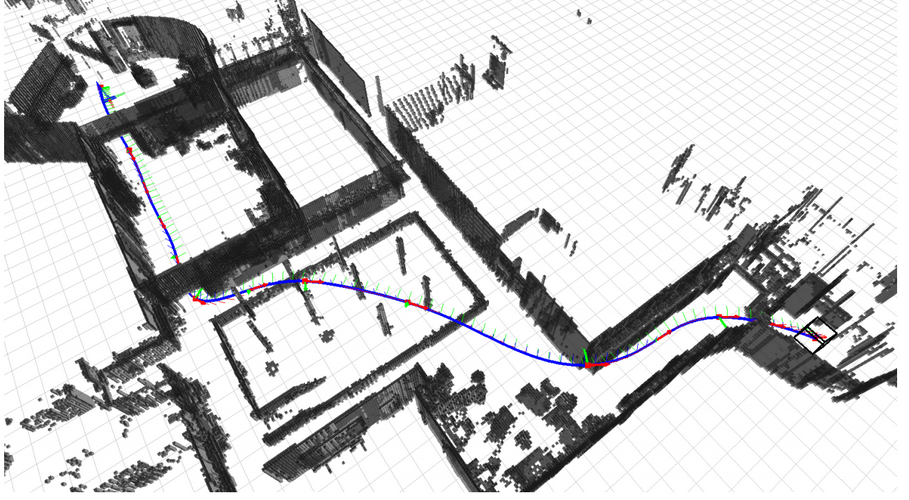
\includegraphics[width=0.6\textwidth]{./images/bry_poly.png}
\caption{Minimum-snap trajectory generation using unconstrained quadratic program. \cite{richter2016polynomial}}
\label{fig:bry_poly}
\end{figure}

\subsection{Sampling-Based Motion Planning}
\label{sec:sampling_planning}
%Gradient-Based Online Safe Trajectory Generation
%for Quadrotor Flight in Complex Environments
Sampling-Based methods perform better in cluttered environments. Some popular sampling based path-planning algorithms include, RRT*, PRM* (Probabilistic Road Map*) and rapidly-exploding random graphs (RRG), which is an extension of RRT. The approach in \cite{webb2013kinodynamic}, the RRT* method is combined with a fixed-final-state-free-final-time controller to obtain asymptotic optimality. Closed-form solutions of optimal trajectories could be derived in this method. 

Bry and Roy et al. \cite{bry2011rapidly} combined the belief roadmap with RRG to address the problem of motion planning in the presence of state uncertainty. The resultant search tree in belief space is provably convergent to the optimal path. Shen et al. \cite{shen2017gradient} used RRG method, along with a trajectory optimization framework, to generate a safe, smooth and dynamically feasible trajectory based on the piecewise line segment initial path. 

\subsection{Search-Based Motion Planning}
\label{sec:search_based_planning}
%Search-based Motion Planning for Quadrotors using
%Linear Quadratic Minimum Time Control
Recent work by Kumar et al. \cite{kumar2017search} aims at computing globally optimum, collision-free, minimum-time, dynamically-feasible trajectories in real-time. When the geometric path is first computed and then smoothened, the generated trajectory may not contain a globally optimum trajectory as this approach does not consider the initial dynamics of the robot. As shown in Figure.~\ref{fig:search_kumar}, the trajectory generated by this approach is superior to other approaches. 

\begin{figure}
\centering
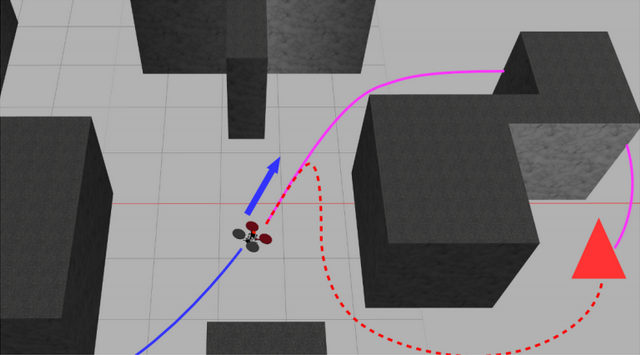
\includegraphics[width=0.6\textwidth]{./images./search_kumar.png}
\caption{Path planning performed at non-zero inital velocity. \cite{kumar2017search} generates the more natural and time optimal magenta curve, where as other approaches gives rise to the red-dashed curve.}
\label{fig:search_kumar}
\end{figure}

Even though others have worked on generating time-optimal trajectories, the algoritms developed were not viable due to their high computation costs. In \cite{kumar2017search}, the algorithm solves an optimal control problem on a set of short-duration motion primitives to explore the space of trajectories. The primitives discretize the state-space into a finite lattice, which is then explored using a graph search algorithm accelerated by a heuristic. 

% Model Predictive Control
\section{Control of Quadrotors}
\label{sec:control_quadrotors}
Due to its recent popularity, practically all the major control techniques have been used to control technique have been treid on quadrotors. Linear control techniques \cite{seigwart2004pid} have been used to control quadrotors by linearizing their dynamics around an operation point, typically the hover position. Better performance is obtained by non-linear control methods like backstepping, sliding mode \cite{seigwart2005backstepping} and feedback linearization \cite{lewis2009dynamic}.

An accurate model of the system is necessary for the above-mentioned control techniques to generate satisfactory results. Modelling errors can considerably deteriorate their performance. Adaptive controllers \cite{kumar2011design} perform well in these cases by correcting the errors in model parameter estimates.

\textit{Model predictive control} (MPC) refers to a set of controllers that use a model to compute inputs from the current time to a future time in order to optimise the behaviour of a model along the input trajectory. Since it is a computationally intensive algorithm, it was used in slow systems like chemical plants and oil refineries. Due to the recent increase in computational capabilities, MPC have become popular in robotics. 

MPC is used to generate trajectories interpolating a given set of way-points \cite{singh2001trajectory} by calculating optimal controls online to minimize a cost function within a receding horizon. The constraints of the problem can be incorporated to the optimal control problem (OCP). In \cite{kamel2015fast}, a fast nonlinear model predictive control (NMPC) approach based on a geometric formulation of the error to track the MAV attitude on the SO(3) special orthogonal group. 

Since the constrained optimization problem is computationally intensive, a trade-off has to be made between time horizon and policy lag. This trade-off is alleviated in \cite{neunert2016fast} by solving an unconstrained MPC problem using Sequential Linear Quadratic (SLQ) solver. By combining trajectory optimization and trajectory contol, this approach generated trajectories of multiple seconds within a few milliseconds.


















